\subsection{Further Reducing the Input Size}

A search is done as \autoref{fig:mnist-dim.pdf}.
When the input size is shrunk to \(8 \times 8\), the misclassifications rate is 15.96\%, which is slightly worse than our target (over 85\% in accuracy).
However, this is a desirable configuration, which means we can fit an input in precisely 8 bytes.
Thus I believe it is worth sacrificing some accuracy here and getting it back using a more aggressive model.

\begin{figure}[ht!]
    \centering
    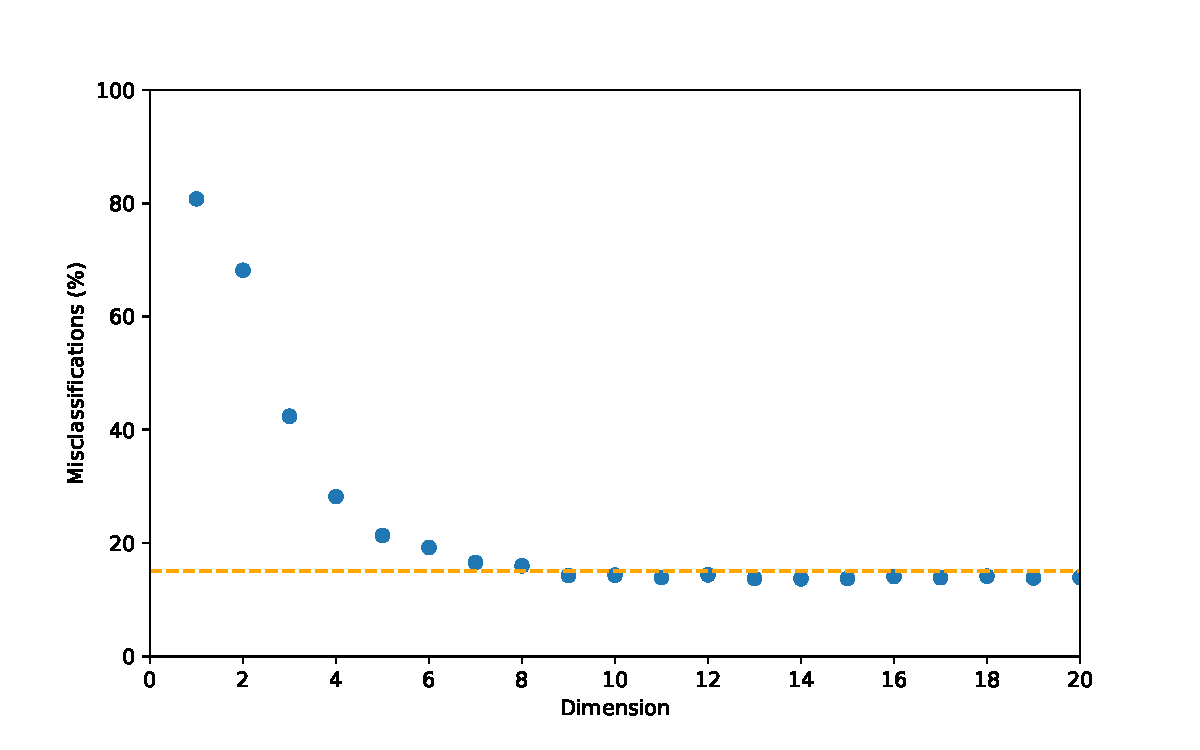
\includegraphics[scale=0.64]{images/mnist-dim.pdf}
    \caption{Misclassifications Rate with floating point numbers under different input size}
    \label{fig:mnist-dim.pdf}
\end{figure}